\subsubsection{TPLAN-DH}

\textbf{TPLAN-DH (TIPO-DE-PLANTA-DÉFICIT-HÍDRICO):} O deficit hídrico tolerável representa a tolerância das plantas à redução do conteúdo de água no solo, mantendo, ainda, sua capacidade de absorção de água.

\begin{table}[h!]
	\centering
	\rowcolors{3}{lightgray}{}
	\caption{Déficit hídrico tolerável para diferentes culturas}
	\label{tab:TPLAN-DH}
	\begin{tabular}{l c}
		\hline \hline
		\multirow{2}{*}{\textbf{Cultura}} & \textbf{Déficit Hídrico Tolerável (\%)} \\
		& \textbf{Gomes(1994)}                    \\
		\hline
		Alface                   & 35                             \\
		Cana-de-açúcar           & 15                             \\
		Feijão                   & 50                             \\
		Laranja                  & 35                             \\
		Melão                    & 20                             \\
		Milho                    & 40                             \\
		Morango                  & 10                             \\
		Tomate                   & 45                             \\
		\hline
	\end{tabular}
\end{table}

Exemplificando para o milho: a absorção de água pelas suas raízes fica comprometida
quando a retirada é maior que 40\% da capacidade de água disponível no solo.

\begin{figure}[h!]
\centering
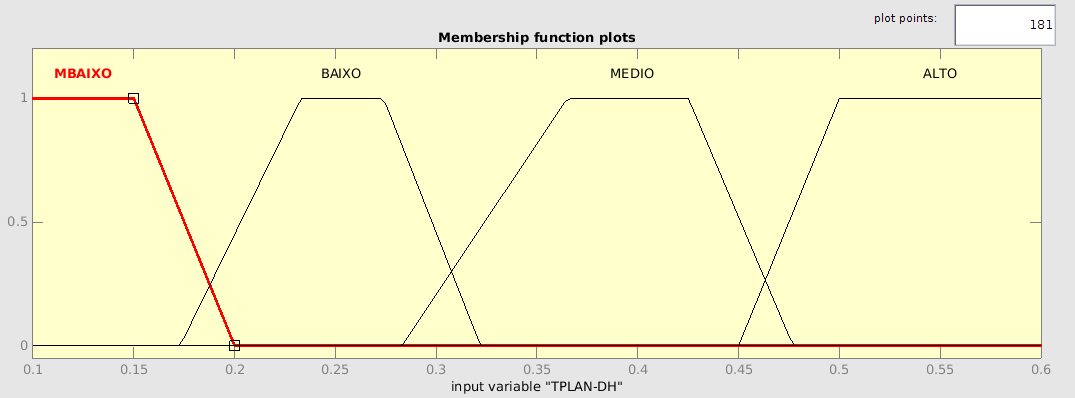
\includegraphics[width=1\linewidth]{Descricao/Imagens/TPLAN-DH}
\caption{Deficit hídrico da planta}
\label{fig:TPLAN-DH}
\end{figure}
